\chapter{Kommuneplan}
En kommuneplan er kommunens overordnede plan for kommunens udvikling. Indenfor en periode på 12 år fastlægger kommunen de overordnede mål og retningslinjer for kommunens udvikling såvel i byerne som i det åbne land. 
\newline
\newline
En kommuneplan består af; en hovedstruktur, retningslinjer, kommuneplanrammer, bilag og tilhørende planredegørelse. 
\newline \indent{     }  Hovedstrukturen er den overordnede, strategiske og sammenfattende fysiske plan for kommunen. Den fastlægger de overordnede mål for udviklingen inden for de enkelte sektorer for hele kommunen og for de enkelte områder. 
\newline \indent{     }  Retningslinjerne udgør de overordnede rammer for kommuneplanlægningen. De fastsætter principperne for arealanvendelsen i kommunen, og danner ligeledes grundlag for kommunens administration af planlovens landzonebestemmelser, samt administrationen af kompetencer indenfor anden lovgivning, herunder natur-, miljø-, bygge- og vejlovgivningen og husdyrloven. Retningslinjerne angiver sammen med områdeudpegningerne hvilke forhold, der skal tages hensyn til i administrationen, og hvilke konkrete skøn der skal foretages for disse områder. 
\newline \indent{     }  Kommuneplanrammerne styrer den overordnede arealanvendelse og danner ramme for indholdet i nye lokalplaner. Planrammerne fastlægger dermed mål, muligheder og begrænsninger for arealanvendelse i de enkelte dele af kommunen. Kommuneplanrammerne har to niveauer: 1) by/bydel/landområde og 2) rammeområder. Det første niveau “by/bydel/landområde”, behandler områdets særlige problemer, værdier og muligheder i en sammenhæng. Det andet niveau “rammeområder”, er det mest detaljerede niveau i kommuneplanen rent geografisk. Her fastsættes de bestemmelser der danner grundlag for lokalplaner.
\newline \indent{     }  Bilag er de generelle rammebestemmelser, hvor der henvises til de aktuelle bilag fra de enkelte emner.
\newline \indent{     }  Planredegørelser beskriver forudsætninger for, og ændringerne i den konkrete planlægning. Byrådet offentliggør, sammen med alle kommuneplanforslag eller med forslag til kommuneplantillæg\footnote{Opstår der problemer med at realisere en lokalplan ud fra kommuneplanen, så anvendes der et kommuneplantillæg, som er et supplement til den eksisterende kommuneplan. Denne kan justere og ændre bestemmelserne i kommuneplanen, for at gøre det muligt at realisere lokalplanen \citep{kommuneplan2009}.}, en redegørelse om planens baggrund og sammenhæng med anden planlægning. Kommuneplanen ledsages også af en planredegørelse og planstrategi, hvilken laves minimum hvert 4. år i tilknytning til kommunens budget. Denne er byrådets instrument og baner vejen for at realisere kommuneplanens mål. Her oplyses blandt andet om kommuneplanens væsentlige forudsætninger, planlægninger der er gennemført det forgangne år, det kommende års kommuneplaninitiativer samt byrådets vurdering af og strategi for udviklingen for både det kommende år (budgetåret), de kommende 4 år (overslagsårene) og en længere periode på 12 år. Desuden laves der jævnligt statusredegørelser, som giver et overordnet billede af kommunens fysiske udvikling og præsenterer de økonomiske tiltag, der knytter sig til kommunens sektorer og geografiske områder \citep{kommuneplan1}.

\section{Aalborg Kommuneplan}
Aalborg Kommuneplan beskriver kommunens udvikling inden for de 12 kommende år og er opdelt i fem fokuspunkter: 
\begin{enumerate}
\item Byerne - et godt sted at bo hele livet
\item Nødvendige forbindelser - mobilitet
\item Det åbne land
\item Bæredygtighedsprofil
\item Aalborg - den attraktive storby
\end{enumerate}
Et af Aalborg Kommuneplans fem fokuspunkter er “Byerne - et godt sted at bo hele livet”. De større byer under Aalborg Kommune har, i kraft af nærheden til Aalborg, en god infrastruktur,  et varieret serviceudbud samt tilstrækkeligt befolkningsunderlag. Det er et særligt potentiale for byvækst, der skal udnyttes for at understøtte Aalborg som Norddanmarks Vækstdynamo. 
\newline \indent{     }  Byvæksten skal have særligt fokus på nye, kreative boligformer, som tilgodeser klimaudfordringer, demografiske udfordringer og bæredygtighed. 
\newline \indent{     }  Ikke kun de større byer nær Aalborg har en væsentlig rolle i projektet. Mindre byer og landsbyer er også i fokus, og har en særlig rolle som opland til Aalborg med store kvaliteter indenfor bosætning, rekreation og friluftsliv.
\newline
\newline
Et andet af Aalborg Kommuneplans fem fokuspunkter er “Nødvendige forbindelser - mobilitet”. Dette fokuspunkt omhandler byens behov for forbindelser, der kan håndtere transportbehovet og gøre det mere attraktivt at benytte offentlig transport såsom bus og tog, samt at tage cyklen, da  Aalborg Kommune har en målsætning om at blive Danmarks førende cykelby. Kommunens mål er færre bilkøer, god adgang til indkøb, service og arbejdspladser samt sikring af forbindelser, der understøtter en effektiv godstransport. Derudover satser Aalborg på en letbane som det bærende element i byen.
\newline
\newline
Fokuspunktet “Det åbne land” omhandler benyttelsen og beskyttelsen af det åbne land. Dette skal ske på et bæredygtigt grundlag med plads til oplevelser, natur, erhvervsinteresser og vedvarende energi. Det åbne land skal danne ramme om levende og aktive områder.
\newline
\newline
Aalborg Kommune har også stor fokus på bæredygtighed og har dertil punktet “Bæredygtighedsprofil”. Udviklingen af et bæredygtigt samfund omhandler flere punkter, såsom at passe på miljøet, klimaet og naturen, om at bygge byer for mennesker og om at få det bedste ud af den nuværende økonomiske virkelighed. En bred tilgang til bæredygtighed er derfor udgangspunktet \citep{kommuneplan2}.

\subsection{Aalborg Vækstakse}
Det femte og sidste fokuspunkt i Aalborgs kommuneplan er “Aalborg - den attraktive storby”. Dette fokuspunkt indeholder yderligere tre punkter; vækstaksen som byens motor, byudviklingsprincipper for Aalborg og fokus på bykvalitet. 
\newline
\newline
Aalborg Kommune har valgt at koncentrere sig om et vækstbånd, kaldet Vækstaksen, som skal danne grundlag for Aalborgs udvikling, hvor der er fokus på det generelle udviklingsprincip. Området går fra Aalborg Lufthavn i vest, gennem midtbyen, til Campus og videre ud til østhavnen, hvilket illustreres på Figur \ref{fig:vaekstakse}. 
\newline \indent{     }  Blandt Vækstaksens mest centrale elementer er færdiggørelsen og videreudviklingen af en række større områder i Aalborg, som for fremtidig skal være med til at skabe Aalborg som storby og præge dens identitet. Gennem disse færdiggørelser vil bykvaliteten øges, og byen vil blive mere attraktiv. Der lægges derfor stor vægt på arkitektoniske overvejelser samt historiske skulpturer og monumenter, når der skal bygges og renoveres. 
\newline \indent{     }  Her har havnefronten, som et af de første områder, gennemgået en stor renovering, hvor der er etableret både Havenebad, Jomfru Ane Parken og sportsfaciliteter. Derudover blev Tivoli Karolinelund fjernet i 2011, og i 2012 åbnede en ny Karolinelund park, som nu danner ramme for mange forskellige nichekulturer, såsom koncerter, Platform 4, legepladser og meget mere, og parken er fortsat under udvikling \citep{jomfruaneparken} \citep{karolinelund}. 
\newline \indent{     }  Aalborg er gennem renoveringen af den nye havnefront også vokset som kulturby, og i dag er kultur blevet en bærende del af byen, hvor der findes KUNSTEN museum, Aalborg Kultur og Kongres center, Nordkraft samt det nye Musikkens Hus, der åbnede i 2014, hvor der hver uge afholdes forskellige koncerter og andre arrangementer. Dette er altsammen med til at styrke Aalborg som vækstby og byens erhvervsturisme. Ligeledes er der planer om en ny kulturbro på Jernbanebroen, som også skal være med til at styrke kulturen i Aalborg og Aalborg Kommune. Ved at styrke kulturen styrkes bykvaliteten også, og byen bliver en levende by, hvor det er muligt at binde shopping, café og kulturliv sammen \citep{kulturbro} \citep{musikkenshus}.
\newline \indent{     }  Den gamle Eternitgrund i Aalborg havde i en lang årrække stået ubrugt hen, men gennem de sidste fem år er der etableret både studieboliger, supermarkeder, fitnesscenter og et nyt legeland for børn. Virksomheder som Plus Bolig og COWI er ligeledes flyttet ned på Eternitten, og i dag er Eternitten blevet en stor drivkraft for Aalborg,  hvor der fortsat  er fremtidige planer om grønne arealer også \citep{eternitten}.
\newline \indent{     }  Projektet om Vækstaksen er i fuld gang, og inden for den nærmeste fremtid skal også Godsbanearealet og det østlige Aalborg udvikles, for at øge oplevelsesmulighederne, kulturtilbudene og skabe attraktive og bæredygtige livsvilkår her. Det er dog ikke kun nybyggerier, som Vækstaksen har fokus på. For Aalborg Kommune er det også vigtigt, at vedligeholde de gamle bygninger, for at opretholde byens historisk identitet.

\begin{figure}[htbp]
	\centering
	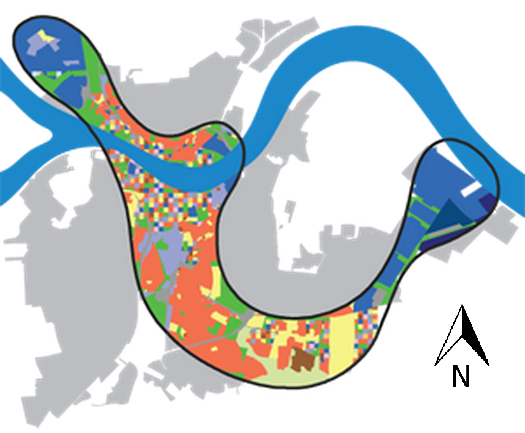
\includegraphics[width=0.5\textwidth]{billeder/vaekstaksen.png}
	\caption{Aalborgs Væsktakse}
	\label{fig:vaekstakse}
\end{figure}

Vækstaksen skal være attraktiv for alle aldersgrupper og skal derfor have noget at tilbyde hver enkelte borger, og skal ligeledes være med til at skabe oplevelsesmuligheder og kulturtilbud.
\newline \indent{     }  En stor del af planerne for Vækstaksen er byfortætning, mobilitet, studieby og miljø. 
Der er i Aalborg Kommune stor udviklingspotentiale inden for byfortætning. På Figur \ref{fig:udvikling} ses udviklingspotentialet i Vækstaksen. De markerede lilla områder er der hvor Aalborg Kommune har bedst udviklingspotentiale.
\newline \indent{     }  Dette udviklingspotentiale er i form af tilbyggelse og omdannelse af boliger, arbejdspladser og naturområder. Byfortætning kan resultere i en meget presset infrastruktur, derfor er mobilitet et essentielt punkt for optimering af byens potentiale. Det er vigtigt, at der er let og hurtigt adgang til offentlig transport, og det skal gøres mere attraktivt, at tage cyklen. Målet er, at få en stor by til at opfattes som en “lille by”, ved at gøre transport lettilgængeligt og derfor nemt at komme fra bydel til bydel. Infrastrukturen vil styrkes blandt andet via en cykelmotorvej samt en kommende letbane, som skal forbinde Østhavnen, Campus, det kommende superhospital i Aalborg Øst, midtbyen og ud til Aalborg Lufthavn.

\begin{figure}[htbp]
	\centering
	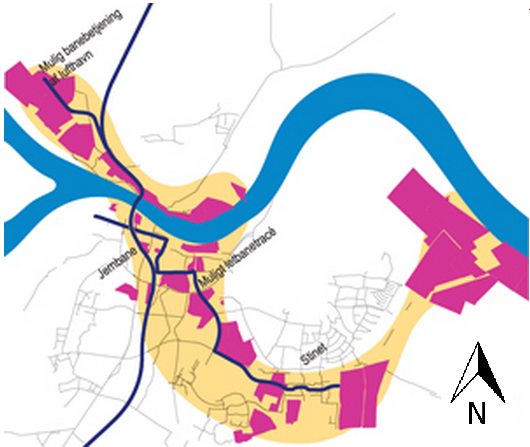
\includegraphics[width=0.5\textwidth]{billeder/udvikling.png}
	\caption{Udviklingspotentiale}
	\label{fig:udvikling}
\end{figure}

Ved Vækstaksens to endepunkter ligger Aalborgs største industriområder, Aalborg Østhavn og Aalborg Lufthavn. Disse industriområder er kommet til, efter industrifirmaer er begyndt at flytte fra havnefronten og ud til yderkanten af Vækstaksen. Trods denne flytning forbliver Aalborg en erhvervsby samtidig med, at den gradvist omdannes til en studieby. De store industrifirmaer er stadig vigtige for Aalborg, da de er med til at skabe omsætning og arbejdspladser. 
\newline \indent{     }  Da Aalborg gradvist omdannes til en studieby, er det vigtigt, at der i Vækstaksen støttes op om Aalborgs studieliv og studiemiljø, da 10\% af Aalborg Kommunes befolkning består af studerende \citep{campus}. Et godt studiemiljø vil styrke innovation, konkurrence og vækst i erhvervslivet. Det er nødvendigt med gode uddannelsesmuligheder, faciliteter samt ungdomsboliger til de studerende, hvilket også vil gøre det attraktivt for udefrakommende at studere i Aalborg. Centrum for studielivet i Aalborg udspringer fra Campus i Aalborg Øst, hvor størstedelen af de videregående uddannelser findes. 
\newline
\newline
Aalborg Kommune ønsker også at udvikle byens natur og udendørsliv. Til at opnå dette vil kommunen opføre parker, stisystemer og vandløb. Vandløbene vil give byen historisk identitet, samtidig med at de vil beskytte byen under eventuel øget vandstand, da de kan forsinke vandet. Formålet med parkerne og et naturrigt Aalborg er at skabe et sundhedsfremmende forhold for alle aldersgrupper og beskytte klimaet. Desuden vil Aalborg Kommune gøre Aalborg til en miljøvenlig storby, hvilket vil gøre byen til en attraktiv by, og dermed øge indbyggertallet. Derfor vil Aalborg Kommune genoprette naturen og give velfærd til byens borgere \citep{kommuneplan3}.

\chapter{Lokalplan}
En lokalplan tager udgangspunkt fra en fremsat kommuneplan, og har til formål at styre udviklingen i et område. Lokalplanen skal give borgerne og byrådet et indblik i et bestemt område og give dem mulighed for at komme med tiltag til den fremlagte plan. Her fastsætter byrådet rammerne for, hvordan arealer, bygninger, beplantning, veje, stier mv. skal anlægges i et givent område. Lokalplaner skal ifølge planloven udformes af byrådet, der har pligt til dette, før der kan gennemføres større bygge- og anlægsprojekter.
\newline
\newline
En lokalplan indeholder punkterne; redegørelse, planbestemmelser og bilag.
\newline \indent{     }  Planen starter med en redegørelse, hvor lokalplanens baggrund og formål fastsættes og hele indholdet fremlægges. Der bliver også redegjort for miljømæssige forhold, hvordan lokalplanen forholder sig til andet byggeri, og om der kræves tilladelser eller anden slags dispensationer fra forskellige myndigheder.  
\newline \indent{     }   I lokalplanen informeres der om planbestemmelser, som er områdets fremtidige anvendelse. Dette illustreres via tekst og billeder.
\newline \indent{     }  Til sidst i lokalplanen ligger alle bilagene. Disse består oftest af forskellige kort (matrikelkort, arealanvendelseskort m.m) samt forskellige tabeller omkring støj fra erhverv og trafik m.m. Bilagene er med til at uddybe og illustrere lokalplanbestemmelserne.
\newline
\newline
Byrådet kan til enhver tid udarbejde et lokalplanforslag. Når et forslag til lokalplanen er udformet, skal det offentliggøres i mindst 8 uger, hvor borgerne kan komme med indsigelser eller forslag til ændringer. Efter de 8 ugers offentliggørelse bedømmer byrådet, hvorvidt eventuelle indsigelser eller ændringer vil blive taget op. Dernæst vedtages planen, hvor den bekendtgøres i avisen og er hermed bindende for ejendommene, som ligger i lokalplanområdet.
\newline \indent{     }  Der må ikke laves ændringer i området i strid med lokalplanen, dog må eksisterende bebyggelser og anvendelse, der er etableret før lokalplanforslagets offentliggørelse, fortsætte. Endvidere er der ikke pligt til at gennemføre tiltag, der beskriver lokalplanen (\citep{lokalplan}, s. 4).

\section{Lokalplan 1-1-107}
Lokalplan 1-1-107 er lokalplanen for området ved Strøybergs Palæ. Lokalplanen er vedtaget af Aalborg Byråd den 12. november 2012, og offentligt bekendtgjort den 21. november 2012 (\citep{lokalplan}, s. 20).
\newline \indent{     }  Området for lokalplanen er ca. 1.200 $m^2$, og ligger ca. 100 m fra Limfjorden. Øst for lokalplanområdet ligger Gammel Havn, mod nord og vest ligger Utzon Parken og mod syd Nyhavnsgade. Ud over Strøybergs Palæ, der ligger i planområdet, er der også enkelte mindre bygninger, garager mm. For at lokalplanen kan blive realiseret, skal mindre bygninger nedrives, hvis de ikke er bevaringsværdige (\citep{lokalplan}, s. 6). Området, som lokalplanen dækker, ses på Figur \ref{fig:1-1-107}.
\newline \indent{     }  Lokalplanen er udarbejdet med et ønske om, at lave en tilbygning til Strøybergs Palæ, hvor anvendelsesmulighederne i området således vil blive ændret til både beboelse, serviceerhverv og kontorerhverv, frem for kun erhverv, som Strøybergs Palæ bliver anvendt til i dag. Lokalplanen er udformet således, at den tager hensyn til, at den nye bebyggelse udformes efter den eksisterende bevaringsværdige bygning, eventuelt med et nutidigt arkitektonisk udtryk, således der er harmoni mellem den nuværende bygning og tilbygningen. Her tages der hensyn til bygningsskala, facaderytme og farve, da Strøybergs Palæ er vurderet til at være en bevaringsværdig bygning med en bevaringsværdi 4 (middel)(\citep{lokalplan}, s. 5 og 9). Bevaringsværdien bestemmes på baggrund af fem værdier; arkitektonisk værdi, kulturhistorisk værdi, miljømæssig værdi, originalitet og tilstand, hvor vurderingen er givet i forhold til helhedsindtrykket af bygningens kvalitet og tilstand, dog vil den arkitektoniske- og den kulturhistoriske værdi veje tungest for bevaringsværdien. Bygninger med bevaringsværdi 2-4 er bygninger, som er fremtrædende grundet deres arkitektur, kulturhistorie og håndværksmæssige udførelse \citep{bevaringsvaerdi}. Lokalplanen fortæller desuden, at tage skal udføres som saddeltage eller som flade tage (\citep{lokalplan}, s. 17).
\newline \indent{     }  Lokalplanen indeholder to delområder, hvor delområdet A er hovedbygningen af Strøybergs Palæ, mens delområde B er sidebygningen dertil og et byggefelt liggende mod nord, hvilket er illustreret på Figur \ref{fig:aogb}. Inden for delområde A må ny bebyggelse opføres i 4 etager, samt en tagetage, og med en kælder maks 1,25 m over terræn, som kan anvendes til parkering, depot og lignende. Inden for delområde B må ny bebyggelse opføres i 3 etager samt en tagetage og med en kælder maks 2 m over terræn. I alt må tilbygningen højst være 19 m høj (\citep{lokalplan}, s. 7).

\begin{figure}[htbp]
	\centering
	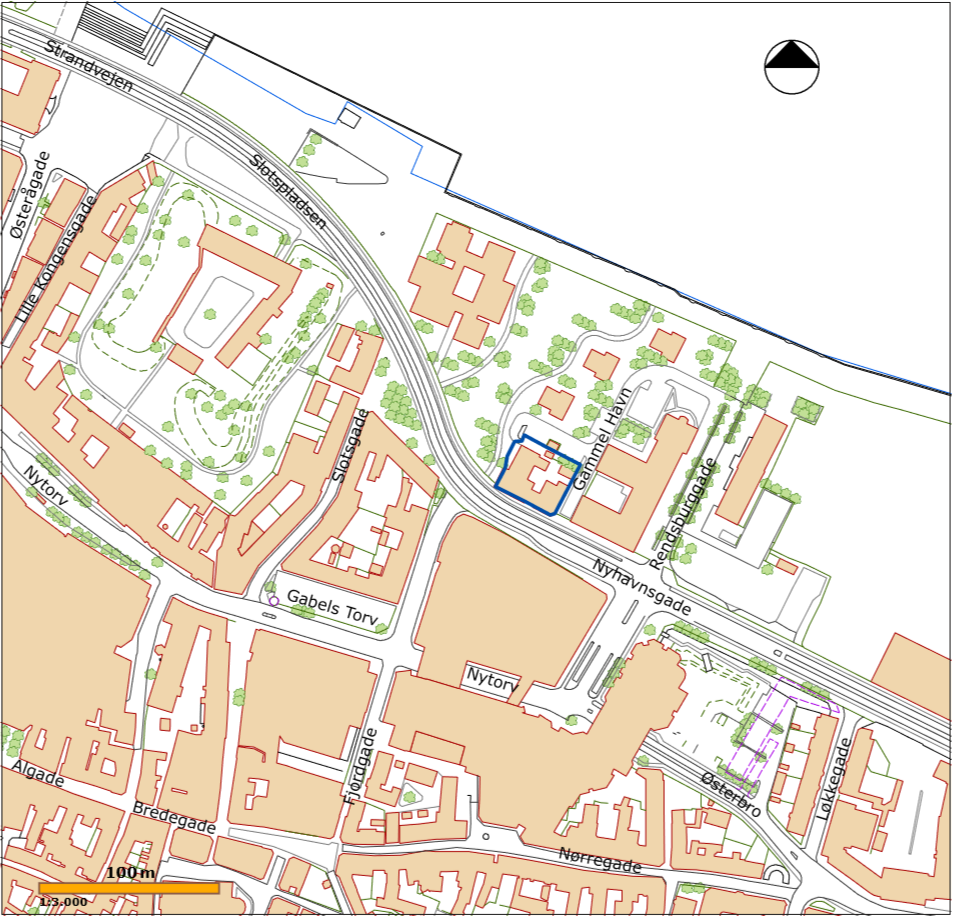
\includegraphics[width=0.5\textwidth]{billeder/nylokalplanoversigt.png}
	\caption{Lokalplan 1-1-107, lokalplanområde}
	\label{fig:1-1-107}
\end{figure}

\begin{figure}[htbp]
	\centering
	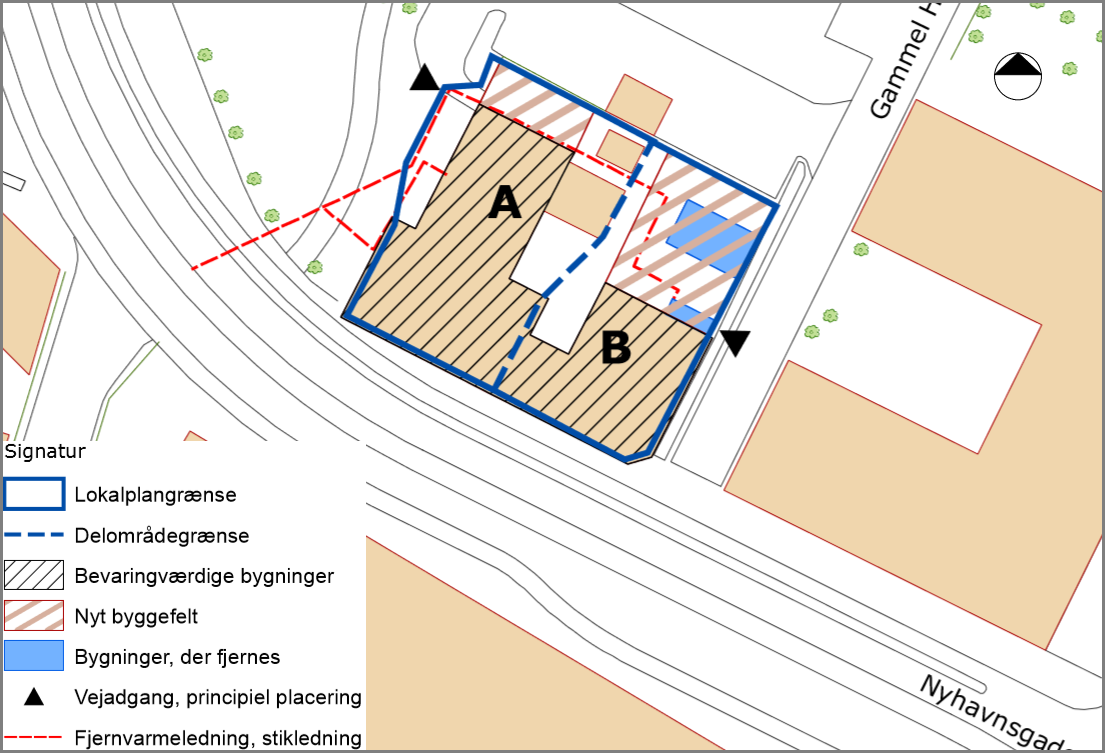
\includegraphics[width=0.5\textwidth]{billeder/signatur.png}
	\caption{Lokalplan 1-1-107, delområde A og B}
	\label{fig:aogb}
\end{figure}

Da lokalplanområdet ligger meget kystnært skal der i større grad dimensioneres efter klimatiske faktorer og ændringer. Her er hovedpunktet vandstandsstigning. Her tages der udgangspunkt fra Aalborg Kommunes klimastrategi. Den forudsiger at den generelle indre vandstand i nordjyske farvande vil kunne stige med op til en meter. Derfor er der fastsat en minimum sokkelkote for stueplan på nye bygninger på 2,36 m DVR 90 grundet risikoen for vandstandsstigning (\citep{lokalplan}, s. 9).
\newline \indent{     }  Bygningen ligger placeret tæt opad detailhandel og erhverv. Området benyttes af kollektiv trafik. Da bygningen ligger placeret ved Nyhavnsgade, kan dette give støjgener fra trafikken. Derfor skal der tages højde for dette, når der bygges. Det indendørs støjniveau må ikke overstige $L_{den}$ 33 dB, og ved udendørs opholdsarealer må den ikke overstige $L_{den}$ 58 dB. Støjisolering skal primært ske indvendigt, så bygningen ikke ændrer udseende. Overholdelse af de forskellige grænseværdier for støj skal kunne dokumenteres, før bygningen må tages i brug (\citep{lokalplan}, s. 8).
Området er kortlagt på vidensniveau 1 og 2 efter jordforureningsloven. Et areal bliver kortlagt på vidensniveau 1, hvis der er kendskab til aktiviteter, der kan forårsage forurening på arealet. Det vil blive kortlagt på vidensniveau 2, hvis der er dokumentation for forurening i jord og grundvand på arealet \citep{vidensniveau}. Hvis der i forbindelse med bygge- og anlægsarbejde konstateres tegn på jordforurening, skal arbejdet standses og kommunens Teknik- og Miljøforvaltning skal underrettes. Herefter vurderes det, om der skal fastsættes vilkår inden arbejdet kan genoptages (\citep{lokalplan}, s. 10).
\newline
\newline
Lokalplanen skal udarbejdes i samspil med den nuværende kommuneplan og anden fysisk planlægning i området omkring. Derfor laves der også tillæg til kommuneplanen, så denne stemmer overens med lokalplanen. Planen er, at der i lokalplanens område kan indrettes et mindre antal boliger. Det forventes at Aalborg Midtby får etableret 2116 nye boliger i perioden 2008-2019. I bygningen kan desuden etableres butikker på maks 250 $m^2$  og 500 $m^2$ pr. etage jf. kommuneplanen (\citep{lokalplan}, s. 8).

\section{Sammenligning af gammel- og ny lokalplan}
I kraft med vedtagelsen af lokalplan 1-1-107 ophæves lokalplanen 10-082 for det område, som lokalplan 1-1-107 omfatter. På trods af, at de to lokalplaner omfatter to forskellige områdestørrelser, så er lokalplanerne fortsat ens på flere punkter, heriblandt miljøforholdene for området. Der er dog nogle små forskelle, og disse forskelle vil blive analyseret i det følgende afsnit. Nedenfor på Figur \ref{fig:10-082} ses lokalplanområdet for lokalplan 10-082

\begin{figure}[htbp]
	\centering
	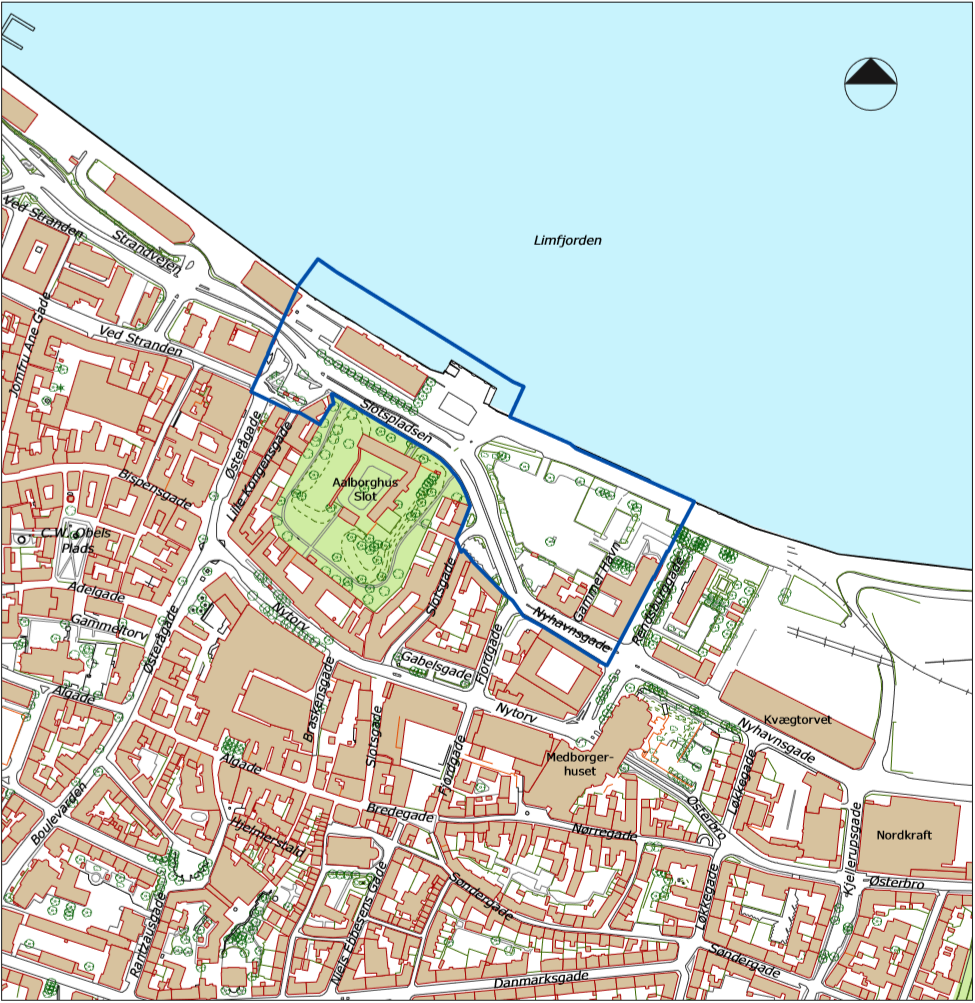
\includegraphics[width=0.5\textwidth]{billeder/lokalplanoversigt.png}
	\caption{Tidligere gældende lokalplan, 10-082, for området}
	\label{fig:10-082}
\end{figure}

I lokalplan 10-082 kan ny bebyggelse for området Strøybergs Palæ bygges i 4 etager plus tagetage med en maks højde på 22 m (\citep{gammellokalplan}, s. 19), hvor der i lokalplan 1-1-107 kan bygges i op til 3 etager plus tagetage for ny bebyggelse med en maks højde på 19 m. Denne ændring i højden kan skyldes, at der har været indsigelser imod de 22 m, da dette muligvis ville fjerne en udsigt eller sollys for de berørte personer. 
\newline \indent{     }  Der er i lokalplan 1-1-107 ligeledes taget højde for vandstandsstigning i Limfjorden, hvilket ikke er gjort i lokalplan 10-082. Grunden til dette kan skyldes, at der ikke tages højde for detaljerne, da lokalplan 10-082 foruden Strøybergs Palæ indeholder tiltag til Utzon Centeret, Slotspladsen og First Slotshotel.
\newline \indent{     }  Ligeledes bliver der præciseret i lokalplan 1-1-107, at isolering for trafikstøj ikke må ændre på facadens udseende, hvor der i lokalplan 10-082 blot står, at enhver ændring på bygningens facade kræver en tilladelse (\citep{gammellokalplan}, s. 19). En grund til at der først i lokalplan 1-1-107 står beskrevet, hvordan isoleringen skal foretages samt at facadeændringer kræver en tilladelse, kan være, at lokalplan 10-082 dækker over et større område end 1-1-107, og at detaljerne på tilbygningen dermed først er relevant for lokalplan 1-1-107. 
\newline \indent{     }  For ny bebyggelse og nye tilbygninger, som er omfattet af lokalplan 1-1-107, gælder det, at nye bygninger skal opføres i overensstemmelse med den eksisterende bebyggelse, dog gerne med nutidig arkitektonisk formsprog. Tilbygninger skal opføres i tilknytning til den eksisterende bevaringsværdige bygning, og skal derfor have det samme arkitektoniske udtryk, som bygningen i forvejen har. 
\newline \indent{     }  Dette punkt i lokalplanen forklarer de overordnede rammer for ny bebyggelse og tilbygning, men udover dette, er det mere frit for det pågældende rådgivningsfirma, at designe og konstruere de pågældende bygninger. De skal blot overholde lokalplanens givne rammer, hvorefter det kan diskuteres og fortolkes, hvor og hvornår grænsen for det arkitektoniske udtryk overskrides. Denne balance er derfor mest op til det rådgivende ingeniørselskab at fortolke.

\section{Diskussion}
Ovenstående afsnit har beskrevet Aalborgs kommuneplan, hvor Vækstaksen er blandt de vigtigste punkter i denne. Aalborg Kommune er i gang med realiseringen af denne, og særligt havnefronten har gennemgået en stor forandring de seneste 5-10 år. 
\newline \indent{     }  Formålet med Vækstaksen er, at styrke Aalborg som by, og der er en forventning fra Aalborg Kommune om, at denne bliver Nordjyllands Vækstdynamo, men er dette realistisk? Nedenstående afsnit vil stille spørgsmålstegn ved Vækstaksen, og diskutere, hvilken sammenhæng Strøybergs Palæ og Vækstaksen har med hinanden. I den forbindelse vil der diskuteres, hvorfor der ønskes en tilbygning, og hvorfor det netop er i dette område, det er fordelagtigt at udvide.
\newline
\newline
\textbf{Vækstaksen - fokus på havnefronten}
\newline
Vækstaksen er placeret således, at den går gennem Aalborgs centrale områder for kultur, uddannelse, erhverv og miljø. Områderne er tæt befolket, og derfor ønsker Aalborg Kommune at etablere en god infrastruktur, som den kommende Letbane eksempelvis skal hjælpe med. Dermed er det fordelagtigt at udvide samt udvikle områderne i Vækstaksen, da de er drivkraften for Aalborg \citep{bedreoverblik}, og det er her, at byens liv er og fremtiden skabes. Selvom områderne i dag fungerer som drivkraft, skal der stadig udvikles i områderne, da Aalborg er en by i stor vækst, hvilket afspejles af både indbyggertal og antal virksomheder, som flytter til og skabes i Aalborg. Derfor kan Aalborg Kommune ikke blot stille sig tilfreds med de nuværende tilstande, da byen skal udvides, for at være forberedt på fremtiden; ellers er der ikke plads til udviklingen, og den vil bremses, gå helt i stå eller i værste fald gå den anden vej.
\newline \indent{     }  Udviklingen vil primært ske gennem en byfortætning, da de centrale områder allerede i dag sprudler med liv gennem kultur, erhverv og uddannelse. Der er altså ikke tale om store udvidelser af områderne, men snarere optimeringer af de allerede eksisterende områder, og derfor kan infrastrukturen opleve problemer. Derfor kan spørgsmålet stilles, om det er realistisk med en fortætning af byen samtidig med, at Aalborg Kommune har en målsætning om, at det skal være let at færdes i byen. Letbanen kan afhjælpe trafikken, men i takt med fortætningen er spørgsmålet, om den er nok, til at det føles let at færdes i Aalborg. Allerede i dag ønskes en tredje Limfjordsforbindelse for køretøjer, da trafikken til og fra Aalborg er tæt i morgentimerne og eftermiddagstimerne, og særligt når der opstår et uheld enten i Limfjordstunnelen eller omkring Limfjordsbroen, hvilke er de to eneste forbindelser for køretøjer over Limfjorden, da den anden forbindelse så bliver overbelastet. 
\newline
\newline
Aalborg har et ønske om at være Danmarks bedste studieby \citep{ungdom}, og derfor kræves der nok studieboliger til de studerende. Der er i landet en generel mangel på studieboliger, og dette gør sig også gældende for Aalborg, selvom det ikke er i ligeså høj grad som eksempelvis København. Det skyldes Aalborgs store fokus på de studerende og behovet for studieboliger, hvoraf der er blevet bygget over 6000 studieboliger siden 2010 inden for Vækstaksen, både på Aalborg og Nørresundby siden, og der bygges fortsat flere nye boliger i dag \citep{studieboliger}. Dette er et led i Vækstaksen og planerne om Aalborgs fremtid, hvilket indtil videre er godt realiseret. De seneste fem år har de videregående uddannelser oplevet rekordmange ansøgninger og dermed flere studerende, hvilket betyder, at studieboligerne hurtigt bliver lejet ud. Et af fokuspunkterne fra Aalborg Kommunes side er, at gøre Aalborg en attraktiv studieby med studievenlige priser på boligerne. Sammenlignes priserne med de tre andre storbyer i Danmark; Aarhus, Odense og København, er boligerne i Aalborg væsentlig billigere, hvilket kan være en medvirkende faktor til, at Aalborg er attraktiv for de unge. Dette punkt fra Vækstaksen er derfor realiseret.
\newline
\newline
Vækstaksen er af stor betydning for Aalborg, og denne udgør en stor del af Aalborg Kommuneplan, og dermed planerne for fremtiden. Flere af punkterne i Vækstaksen er beskrevet ovenfor, men her har fokus været på studerende samt infrastrukturen. Aalborg Kommune har også et ønske om, at byen skal være for alle mennesker i alle aldersgrupper samt et attraktivt sted for erhverv. Spørgsmålet er dog, hvor erhverv skal etableres inden for Vækstaksen, og hvad der kan gøres for de indbyggere, som ikke er studerende. Ses der på naturområderne og de mange attraktioner i byen, så er disse for alle aldersgrupper, men havnefronten, som er en af de bærende elementer i Vækstaksen, anvendes primært af unge mennesker, og der er ikke meget, der indbyder til familier med børn eller for den ældre generation. For at Vækstaksen skal få den betydning, som Aalborg Kommune ønsker, er det nødvendigt med flere tiltag for den ældre aldersgruppe. 
\newline \indent{     }  For nye virksomheder gælder det, at der skal være nok kontorlokaler og bygninger, som kan husere virksomhederne. Ligeledes skal virksomhedens interesserer gerne falde ind med Aalborg og passe sammen, således at der også kommer kunder til blandt Aalborgs befolkning. Med en målsætning om, at være en attraktiv storby med mange muligheder for virksomheder, er der derfor gode muligheder for at drive virksomhed i Aalborg, også for fremtiden. Indenfor Vækstaksens bælte ligger der utallige af virksomheder, men der er stadig både tomme erhvervslokaler og planer om udvidelser af allerede eksisterende lokaler, som vil give plads til flere virksomheder. Heriblandt skal der ske en udvidelse af Strøybergs Palæ, som har en central beliggenhed i Vækstaksen, helt nede ved havnefronten. 
\newline
\newline
\textbf{Hvorfor udvide Strøybergs Palæ?}
\newline
Strøybergs Palæ ligger i Vækstaksen. På Figur \ref{fig:udvikling} ses det, at Strøybergs Palæ ligger i det lilla område og er dermed i et område, hvor der er størst mulighed for udvikling inden for Vækstaksen. På grund af havnefrontens udvikling de sidste 10 år, har der været fokus på udviklingen her, og nu har Aalborg Kommune ment, at det er på tide at udvikle området ved Strøybergs Palæ, da der allerede er bygget Musikkens Hus, havnefronten, Utzon Centeret og Utzon Parken omkring området. Udviklingen omkring havnefronten er sket i takt med Vækstaksens fokus herpå. Om havnefronten havde fået en udvikling overhovedet eller i lige så høj grad, hvis tankerne og ideérne omkring Vækstaksen ikke var blevet sat i værk, kan diskuteres. Strøybergs Palæ havde måske aldrig været et relevant emne at tage op i forhold til udviklingen af Aalborg, hvis ikke bygningen havde ligget i Vækstaksen. Havde Vækstaksen ligget anderledes, således Strøybergs Palæ lå uden for Vækstaksen, var det måske aldrig kommet på tale, at lave en tilbygning hertil, men blot lade den stå som den er. Placeringen af Strøybergs Palæ midt i Vækstaksen, må formodes at have haft indflydelse på beslutningen om, at der skal laves en tilbygning, fordi bygningen skal leve op til Aalborg Kommunes forventninger og ønsker for fremtiden, og fordi de nok mener, at der er udviklingspotentiale gennem denne bygning også. Tilbygningen kan bruges til erhvervslokaler, og dette vil kunne tiltrække en eller flere nye virksomheder til området, og dermed udvikle både området og Aalborg by. Her kan spørgsmålet dog også stilles, om denne tilbygning vil få den ønskede effekt og kunne leve op til disse målsætninger. Det vil være naivt at tro, at en udvidelse på nogle få hundrede kvadratmeter vil gøre en betydende forskel for Aalborg og Vækstaksen, og det kan derfor ikke alene være grunden til tilbygningen, men snarere en af flere årsager. Strøybergs Palæ er kun en lille del af Vækstaksen, og skal derfor ikke bære Aalborgs udvikling og vækst alene.
\newline \indent{     }  Hovedpunkterne i Vækstaksen er, at Aalborg skal vokse som by, og udvikles gennem en byfortætning, hvor målet er, at flere virksomheder og indbyggere kommer til byen. En udvidelse af Strøybergs Palæ vil betyde et ekstra antal erhvervslokaler, og dette passer godt sammen med Vækstaksen. Tilbygningen betyder desuden, at Strøybergs Palæ vil få et mere harmonisk udseende ud mod vandet, da tilbygningen vil blive bygget i samme stil som resten af bygningen, og den nordlige del af bygningen nu vil komme op i ca. samme højde, som resten af bygningen. Sammen med resten af havnefronten vil Strøybergs Palæ derfor gennemgå en renovering, som løfter udseendet samt medfører at området nu har en mere ensformet og harmonisk stil. 
\newline \indent{     }  Det, at området bliver et centralt fokuspunkt for fremtiden betyder også, at området bliver mere attraktivt, idét der kommer til at ske en fortsat udvikling af området, og netop derfor kan en tilbygning være en god investering, da det giver ekstra plads og bedre forudsætninger for udviklingen.